\begin{figure}[t]
\centering
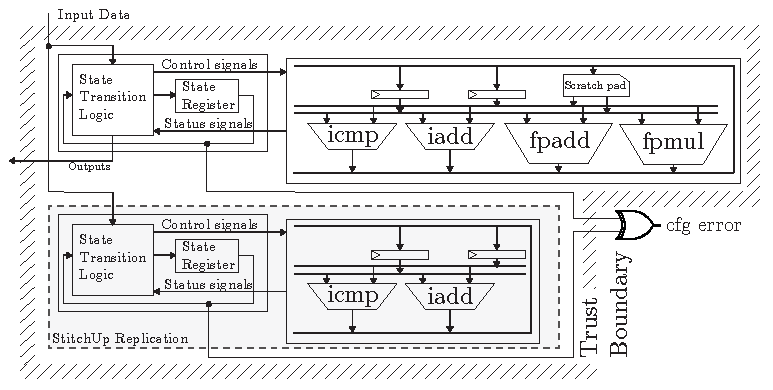
\includegraphics[width=3.5in]{./imgs/StitchUpReplication.pdf}
\caption{Default circuit (a) and Control Replicant (b) for our Dot Product example in Listing \ref{lst:DotProduct}, with Trust Boundary \vspace{-5mm}}
\label{fig:HLSArch}
\end{figure}

A Soft Error or Single Event Upset is a random, non-catastrophic error, where radiation causes
a perturbation to a circuit by temporarily altering a single signal or datum.
Detecting and mitigating such errors is important in some fields, such as satellite design,
where high design costs, harsh environments, and the difficulties in repairing once deployed make it necessary.
Additionally, due to the continuing increase in semiconductor density, the current soft error challenges 
experienced in space will also occur in future terrestrial devices.\cite{normand1996single}\cite{henkel2013reliable}.

FPGA devices work by mapping circuit descriptions into a collection of Logic Elements,
which are described in programmable Look-Up-Tables (LUTs) and routed together via
programmable switchboxes.
Configuration data for both the look-up-tables and switchboxes are stored in an SRAM based
configuration memory, which means soft errors can either change the functionality
of Logic Elements or can change the routing between them.
Other memories called block memory and flip-flops are also present in FPGA devices,
and soft errors in these regions can cause transient errors in the circuit.

%How this changes the protection strategy compared to software and VLSI
For ASIC designs, registers are the most vulnerable to soft-errors with
combinational logic contributing very little to overall circuit relability \cite{baumann2005soft}.
This makes ASIC approaches which analyses and protect vulnerable registers, such as in \cite{chen2014reliability},
promising approaches.
However in FPGA devices the most vulnerable region is the SRAM based configuration memory,
so such approaches would have little impact requiring methods that perform combinatorial logic
replication, such as StitchUp or DMR/TMR.

%ECC and frame based checking approaches
Circuits described within configuration memory are usually protected in one of two ways:
(1)the circuit is replicated with comparison; (2)ECC/CRC signals associated with
frames of the configuration memory are regularly scanned for errors.
Replication uses extra area and power but has low error detection latency and can
protect both configuration memory and registers,
while ECC/CRC checks consume less area and power in exchange for higher detection 
latency and an inability to protect registers.

For this paper our \emph{fault model} assumes that a single soft error
can occur at most every clock cycle, and that this error can effect block memory,
SRAM configuration memory, or flip-flops.
Since errors are not solely within the configuration memory, replication must be used,
as configuration ECC/CRC cannot protect the registers in our control structure.
Figure \ref{fig:HLSArch} shows a StitchUp generated circuit for the dot product 
example in Listing \ref{lst:DotProduct}, with the original circuit on top and the
control-flow structure shadow beneath it.
StitchUp aims to protect all configuration, block, and Flip-flop bits within the
trust boundary (grey box) as everything outside, such as routing to
external I/O or DDR, is not protected.

